%% bare_conf.tex
%% V1.4b
%% 2015/08/26
%% by Michael Shell
%% See:
%% http://www.michaelshell.org/
%% for current contact information.
%%
%% This is a skeleton file demonstrating the use of IEEEtran.cls
%% (requires IEEEtran.cls version 1.8b or later) with an IEEE
%% conference paper.
%%
%% Support sites:
%% http://www.michaelshell.org/tex/ieeetran/
%% http://www.ctan.org/pkg/ieeetran
%% and
%% http://www.ieee.org/

%%*************************************************************************
%% Legal Notice:
%% This code is offered as-is without any warranty either expressed or
%% implied; without even the implied warranty of MERCHANTABILITY or
%% FITNESS FOR A PARTICULAR PURPOSE! 
%% User assumes all risk.
%% In no event shall the IEEE or any contributor to this code be liable for
%% any damages or losses, including, but not limited to, incidental,
%% consequential, or any other damages, resulting from the use or misuse
%% of any information contained here.
%%
%% All comments are the opinions of their respective authors and are not
%% necessarily endorsed by the IEEE.
%%
%% This work is distributed under the LaTeX Project Public License (LPPL)
%% ( http://www.latex-project.org/ ) version 1.3, and may be freely used,
%% distributed and modified. A copy of the LPPL, version 1.3, is included
%% in the base LaTeX documentation of all distributions of LaTeX released
%% 2003/12/01 or later.
%% Retain all contribution notices and credits.
%% ** Modified files should be clearly indicated as such, including  **
%% ** renaming them and changing author support contact information. **
%%*************************************************************************


% *** Authors should verify (and, if needed, correct) their LaTeX system  ***
% *** with the testflow diagnostic prior to trusting their LaTeX platform ***
% *** with production work. The IEEE's font choices and paper sizes can   ***
% *** trigger bugs that do not appear when using other class files.       ***                          ***
% The testflow support page is at:
% http://www.michaelshell.org/tex/testflow/



\documentclass[conference]{IEEEtran}
% Some Computer Society conferences also require the compsoc mode option,
% but others use the standard conference format.
%
% If IEEEtran.cls has not been installed into the LaTeX system files,
% manually specify the path to it like:
% \documentclass[conference]{../sty/IEEEtran}





% Some very useful LaTeX packages include:
% (uncomment the ones you want to load)


% *** MISC UTILITY PACKAGES ***
%
% \usepackage{ifpdf}
% Heiko Oberdiek's ifpdf.sty is very useful if you need conditional
% compilation based on whether the output is pdf or dvi.
% usage:
% \ifpdf
%   % pdf code
% \else
%   % dvi code
% \fi
% The latest version of ifpdf.sty can be obtained from:
% http://www.ctan.org/pkg/ifpdf
% Also, note that IEEEtran.cls V1.7 and later provides a builtin
% \ifCLASSINFOpdf conditional that works the same way.
% When switching from latex to pdflatex and vice-versa, the compiler may
% have to be run twice to clear warning/error messages.






% *** CITATION PACKAGES ***
%
\usepackage{cite}
% cite.sty was written by Donald Arseneau
% V1.6 and later of IEEEtran pre-defines the format of the cite.sty package
% \cite{} output to follow that of the IEEE. Loading the cite package will
% result in citation numbers being automatically sorted and properly
% "compressed/ranged". e.g., [1], [9], [2], [7], [5], [6] without using
% cite.sty will become [1], [2], [5]--[7], [9] using cite.sty. cite.sty's
% \cite will automatically add leading space, if needed. Use cite.sty's
% noadjust option (cite.sty V3.8 and later) if you want to turn this off
% such as if a citation ever needs to be enclosed in parenthesis.
% cite.sty is already installed on most LaTeX systems. Be sure and use
% version 5.0 (2009-03-20) and later if using hyperref.sty.
% The latest version can be obtained at:
% http://www.ctan.org/pkg/cite
% The documentation is contained in the cite.sty file itself.






% *** GRAPHICS RELATED PACKAGES ***
%
\ifCLASSINFOpdf
   \usepackage[pdftex]{graphicx}
  % declare the path(s) where your graphic files are
  % \graphicspath{{../pdf/}{../jpeg/}}
  % and their extensions so you won't have to specify these with
  % every instance of \includegraphics
   \DeclareGraphicsExtensions{.pdf,.jpeg,.png}
\else
  % or other class option (dvipsone, dvipdf, if not using dvips). graphicx
  % will default to the driver specified in the system graphics.cfg if no
  % driver is specified.
   \usepackage[dvips]{graphicx}
  % declare the path(s) where your graphic files are
   \graphicspath{{../eps/}}
  % and their extensions so you won't have to specify these with
  % every instance of \includegraphics
   \DeclareGraphicsExtensions{.eps}
\fi
% graphicx was written by David Carlisle and Sebastian Rahtz. It is
% required if you want graphics, photos, etc. graphicx.sty is already
% installed on most LaTeX systems. The latest version and documentation
% can be obtained at: 
% http://www.ctan.org/pkg/graphicx
% Another good source of documentation is "Using Imported Graphics in
% LaTeX2e" by Keith Reckdahl which can be found at:
% http://www.ctan.org/pkg/epslatex
%
% latex, and pdflatex in dvi mode, support graphics in encapsulated
% postscript (.eps) format. pdflatex in pdf mode supports graphics
% in .pdf, .jpeg, .png and .mps (metapost) formats. Users should ensure
% that all non-photo figures use a vector format (.eps, .pdf, .mps) and
% not a bitmapped formats (.jpeg, .png). The IEEE frowns on bitmapped formats
% which can result in "jaggedy"/blurry rendering of lines and letters as
% well as large increases in file sizes.
%
% You can find documentation about the pdfTeX application at:
% http://www.tug.org/applications/pdftex





% *** MATH PACKAGES ***
%
\usepackage{amsmath}
% A popular package from the American Mathematical Society that provides
% many useful and powerful commands for dealing with mathematics.
%
% Note that the amsmath package sets \interdisplaylinepenalty to 10000
% thus preventing page breaks from occurring within multiline equations. Use:
%\interdisplaylinepenalty=2500
% after loading amsmath to restore such page breaks as IEEEtran.cls normally
% does. amsmath.sty is already installed on most LaTeX systems. The latest
% version and documentation can be obtained at:
% http://www.ctan.org/pkg/amsmath





% *** SPECIALIZED LIST PACKAGES ***
%
%\usepackage{algorithmic}
% algorithmic.sty was written by Peter Williams and Rogerio Brito.
% This package provides an algorithmic environment fo describing algorithms.
% You can use the algorithmic environment in-text or within a figure
% environment to provide for a floating algorithm. Do NOT use the algorithm
% floating environment provided by algorithm.sty (by the same authors) or
% algorithm2e.sty (by Christophe Fiorio) as the IEEE does not use dedicated
% algorithm float types and packages that provide these will not provide
% correct IEEE style captions. The latest version and documentation of
% algorithmic.sty can be obtained at:
% http://www.ctan.org/pkg/algorithms
% Also of interest may be the (relatively newer and more customizable)
% algorithmicx.sty package by Szasz Janos:
% http://www.ctan.org/pkg/algorithmicx




% *** ALIGNMENT PACKAGES ***
%
%\usepackage{array}
% Frank Mittelbach's and David Carlisle's array.sty patches and improves
% the standard LaTeX2e array and tabular environments to provide better
% appearance and additional user controls. As the default LaTeX2e table
% generation code is lacking to the point of almost being broken with
% respect to the quality of the end results, all users are strongly
% advised to use an enhanced (at the very least that provided by array.sty)
% set of table tools. array.sty is already installed on most systems. The
% latest version and documentation can be obtained at:
% http://www.ctan.org/pkg/array


% IEEEtran contains the IEEEeqnarray family of commands that can be used to
% generate multiline equations as well as matrices, tables, etc., of high
% quality.




% *** SUBFIGURE PACKAGES ***
%\ifCLASSOPTIONcompsoc
%  \usepackage[caption=false,font=normalsize,labelfont=sf,textfont=sf]{subfig}
%\else
%  \usepackage[caption=false,font=footnotesize]{subfig}
%\fi
% subfig.sty, written by Steven Douglas Cochran, is the modern replacement
% for subfigure.sty, the latter of which is no longer maintained and is
% incompatible with some LaTeX packages including fixltx2e. However,
% subfig.sty requires and automatically loads Axel Sommerfeldt's caption.sty
% which will override IEEEtran.cls' handling of captions and this will result
% in non-IEEE style figure/table captions. To prevent this problem, be sure
% and invoke subfig.sty's "caption=false" package option (available since
% subfig.sty version 1.3, 2005/06/28) as this is will preserve IEEEtran.cls
% handling of captions.
% Note that the Computer Society format requires a larger sans serif font
% than the serif footnote size font used in traditional IEEE formatting
% and thus the need to invoke different subfig.sty package options depending
% on whether compsoc mode has been enabled.
%
% The latest version and documentation of subfig.sty can be obtained at:
% http://www.ctan.org/pkg/subfig




% *** FLOAT PACKAGES ***
%
%\usepackage{fixltx2e}
% fixltx2e, the successor to the earlier fix2col.sty, was written by
% Frank Mittelbach and David Carlisle. This package corrects a few problems
% in the LaTeX2e kernel, the most notable of which is that in current
% LaTeX2e releases, the ordering of single and double column floats is not
% guaranteed to be preserved. Thus, an unpatched LaTeX2e can allow a
% single column figure to be placed prior to an earlier double column
% figure.
% Be aware that LaTeX2e kernels dated 2015 and later have fixltx2e.sty's
% corrections already built into the system in which case a warning will
% be issued if an attempt is made to load fixltx2e.sty as it is no longer
% needed.
% The latest version and documentation can be found at:
% http://www.ctan.org/pkg/fixltx2e


%\usepackage{stfloats}
% stfloats.sty was written by Sigitas Tolusis. This package gives LaTeX2e
% the ability to do double column floats at the bottom of the page as well
% as the top. (e.g., "\begin{figure*}[!b]" is not normally possible in
% LaTeX2e). It also provides a command:
%\fnbelowfloat
% to enable the placement of footnotes below bottom floats (the standard
% LaTeX2e kernel puts them above bottom floats). This is an invasive package
% which rewrites many portions of the LaTeX2e float routines. It may not work
% with other packages that modify the LaTeX2e float routines. The latest
% version and documentation can be obtained at:
% http://www.ctan.org/pkg/stfloats
% Do not use the stfloats baselinefloat ability as the IEEE does not allow
% \baselineskip to stretch. Authors submitting work to the IEEE should note
% that the IEEE rarely uses double column equations and that authors should try
% to avoid such use. Do not be tempted to use the cuted.sty or midfloat.sty
% packages (also by Sigitas Tolusis) as the IEEE does not format its papers in
% such ways.
% Do not attempt to use stfloats with fixltx2e as they are incompatible.
% Instead, use Morten Hogholm'a dblfloatfix which combines the features
% of both fixltx2e and stfloats:
%
% \usepackage{dblfloatfix}
% The latest version can be found at:
% http://www.ctan.org/pkg/dblfloatfix




% *** PDF, URL AND HYPERLINK PACKAGES ***
%
\usepackage{url}
% url.sty was written by Donald Arseneau. It provides better support for
% handling and breaking URLs. url.sty is already installed on most LaTeX
% systems. The latest version and documentation can be obtained at:
% http://www.ctan.org/pkg/url
% Basically, \url{my_url_here}.


\usepackage{caption}
\usepackage{subcaption}


% *** Do not adjust lengths that control margins, column widths, etc. ***
% *** Do not use packages that alter fonts (such as pslatex).         ***
% There should be no need to do such things with IEEEtran.cls V1.6 and later.
% (Unless specifically asked to do so by the journal or conference you plan
% to submit to, of course. )


% correct bad hyphenation here
\hyphenation{op-tical net-works semi-conduc-tor}


\begin{document}
%
% paper title
% Titles are generally capitalized except for words such as a, an, and, as,
% at, but, by, for, in, nor, of, on, or, the, to and up, which are usually
% not capitalized unless they are the first or last word of the title.
% Linebreaks \\ can be used within to get better formatting as desired.
% Do not put math or special symbols in the title.
\title{Team Solaria COMP9517 Project}


% author names and affiliations
% use a multiple column layout for up to three different
% affiliations
\author{\IEEEauthorblockN{Yishun Jin}
\IEEEauthorblockA{yishun.jin@student.unsw.edu.au\\
z5235653}
\and
\IEEEauthorblockN{Wei Wang}
\IEEEauthorblockA{wei.wang.1@student.unsw.edu.au\\
z5200638}
\and
\IEEEauthorblockN{Yue He}
\IEEEauthorblockA{yue.he1@student.unsw.edu.au\\
z5243835}
\and
\IEEEauthorblockN{Mingxi Shen}
\IEEEauthorblockA{mingxi.shen@student.unsw.edu.au\\
z5243140}
\and
\IEEEauthorblockN{Mingqian Lin}
\IEEEauthorblockA{mingqian.lin@student.unsw.edu.au\\
z5240524}
\and
}


\maketitle
\IEEEpeerreviewmaketitle



\section{Introduction}

Our project aims to finish three tasks

\begin{enumerate}
\item Locate the plants on the tray.
\item Segment the plants from the background.
\item Leaf segmentation.
\end{enumerate}

All the tasks are using the Plant Phenotyping Dataset. This dataset provides us with images, foreground, and the leaf segmentation. So we can evaluate all the tasks after finished each one. All the tasks are using different methods, and these methods will be explained in the following content.


\section{Literature Review}

Task 1 uses color extraction to deal with these photos. The photos of different images are shot in different environment, and also, they are not in the same size, it means that we may have to use different parameters while treating these three datasets. Also, we should think carefully on what kind of color space to use. For example, hsv or rgblab.

The task 2 uses the combination of color extraction and image denoising to do the segmentation. Suitable image segmentation techniques are key technologies to solve the problem \cite{pal1993review}. Previous research has established that mean shift algorithm has good performance for image segmentation, while watershed algorithm also has tremendous benefits. Mean shift algorithm, like the K-Means algorithm, is a clustering algorithm based on clustering centers. The difference is that the final clustering effect of the Mean Shift algorithm is not affected by the initial cluster center. Essentially, it is a kernel density estimation algorithm that moves each point to the local maximum point of the density function, which has achieved many successful applications in the field of image segmentation, such as tracking vehicle changing in size \cite{peng2005automatic}. Watershed algorithm is also a typical image region segmentation method. Its basic idea is to treat the gray value of each pixel in the image as altitude, the boundary of each local minimum and its influence area is called a watershed. Then connect the pixels with similar spatial positions and similar gray values to form a closed contour. There are relatively studies in the area of PET images segmentation \cite{riddell1999watershed}.

For task 3, we used instance segmentation \cite{Hafiz_2020} which is an approach that identifies, for every pixel, a belonging instance of the object. There are many ways to approach instance segmentation, for example, K-Means clustering algorithm, histogram-based methods, edge detection, and also deep learning methods. The segmentation of the foreground can be achieved using non-machine learning method. But when it comes to the segmentation of leaves inside of the foreground, most methods available are usually machine learning methods. Therefore, to achieve the goal, we used a deep learning framework from facebook called  \textbf{Detectron2}. 

\section{Methods}

\subsection{Task 1 Color Extraction and Find Contour}

We use four steps to separate green color from the background.
Step one, we convert images’ color space into hsv. Step two, we use \verb|cv2.inRange| function to extract green color. Step three, we turn the output of step two into grayscale image. Step four, \verb|cv2.findCounters| function is used to find rectangles.
Of course, above are just an ideal experiment process. Filtering noise is the biggest challenge. To get rid of interference of noise, we set a dynamic boundary of rectangles' size. We choose top 30 largest rectangles and calculate the average size. For Ara2012 dataset, we choose average size/4 to be the lower limit of rectangles' area, and for the rest two datasets, we choose 1/25 average size. This is because plants in Ara2012 are almost same in size while plants’ sizes in Canon and RPi are very different. Some plants are small and even not growing, some plants are big and growing rapidly, this makes average size/4 much bigger than baby plants, so we have to reduce the lower limit to average size/25.
Although all the baby plants can be detected by reducing the lower limit, moss will also be included. Because of this, we have to think of a way to filter out moss. As moss is always connected together, it will cover most area of the rectangle while plants only cover below 60\% area of the rectangle, so we calculate the mean value of rectangle’s blue channel, and find that moss always has higher value than plants. After setting a parameter to limit the upper bound of rectangle’s mean value on blue channel, we finally get a good result.

\subsection{Task 2 Image Segmentation}
The task 2 uses two techniques: color space and image denoising.

\subsubsection{Color Space}
Color space is an abstract mathematical model that uses a set of values to represent colors. Generally, RGB is the color space we use the most - an image is represented by three channels, namely red (R), green (G) and blue (B). Combining these three colors in different forms can form almost all other colors. Nevertheless, the RGB model is not intuitive enough to continuously change colors, usually all attribute values have to be changed. Besides, RGB is greatly affected by brightness. Therefore, RGB color space is suitable for image display, but not very suitable for image processing. Compared to RGB, HSV color space is more frequently used in image processing. HSV expresses color image by three parts: Hue, Saturation, Value. HSV model is shown in figure \ref{fig_HSV_model}

\begin{figure}
    \centering
    \includegraphics[]{img/hsv.jpg}
    \caption{The HSV Model}
    \label{fig_HSV_model}
\end{figure}

\subsubsection{Image Denoising}
Image denoising methods have always been a research focus in image processing. Unfortunately, the current denoising algorithm does not have a perfect solution in practical applications \cite{buades2005review}. There are usually different denoising methods for different noises. In this task, there may be some other small plants in the soil after the green is extracted. We need to remove it as much as possible. Common denoising methods include mean filtering, Gaussian filtering, and median filtering. 


\subsection{Task 3 Instance Segmentation}

It is a multi-instance segmentation problem. We use \textbf{Detectron 2}\cite{wu2019detectron2} which is FAIR's next-generation platform for object detection and segmentation. And we use \textbf{Mask-RCNN}\cite{He_2017} to approach our instance segmentation.

\textbf{Mask R-CNN} is a great solution for instance segmentation. It can be easily considered as ResNet-FPN + Fast-RCNN + mask.

\begin{figure}[h!]
\centering
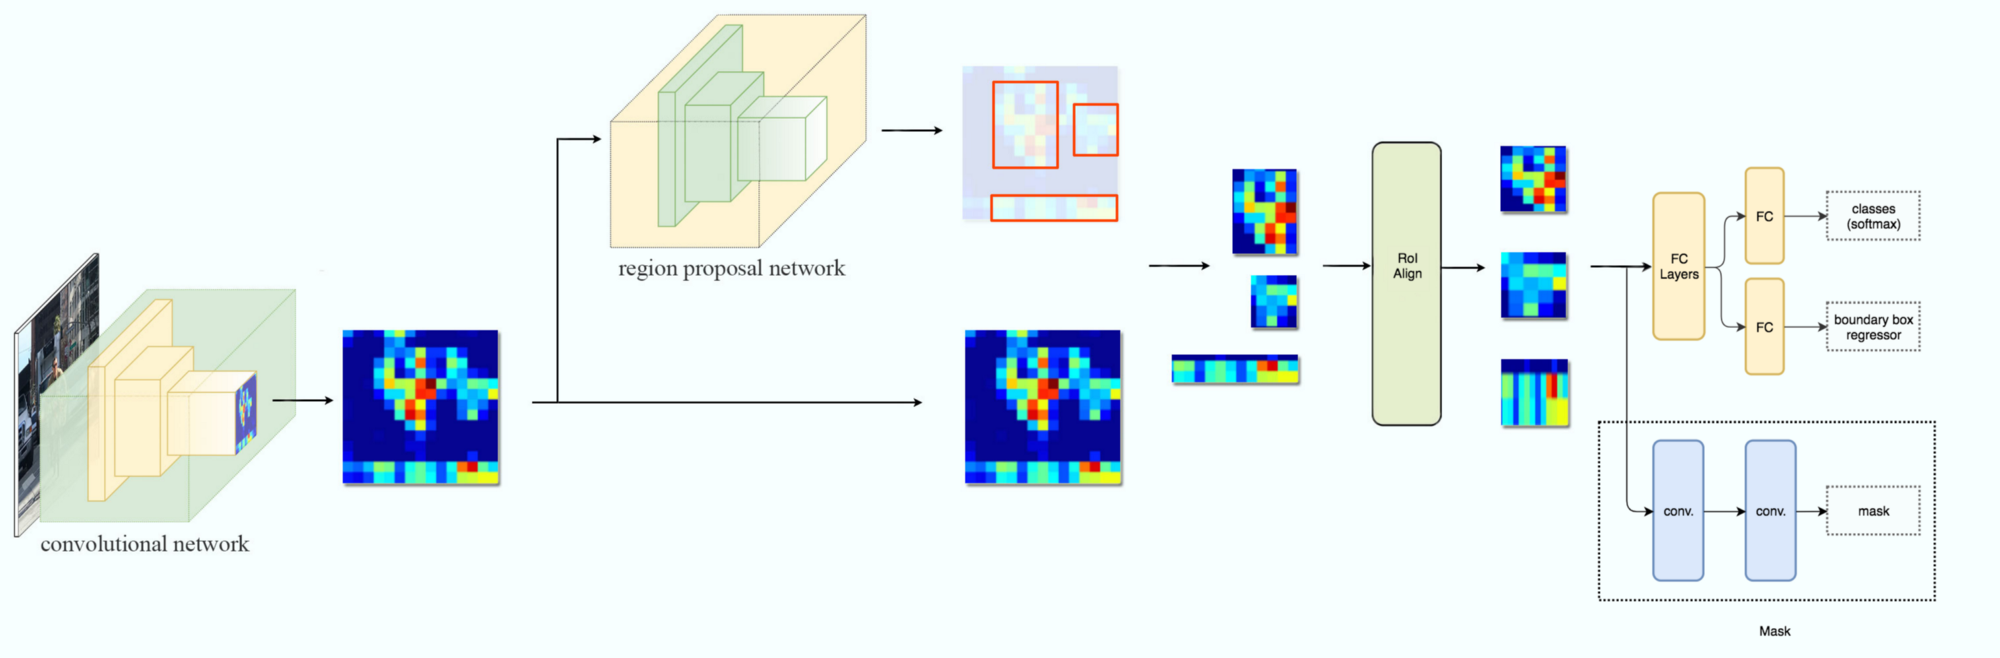
\includegraphics[width=\linewidth]{img/maskrcnn.png}
\caption{Mask R-CNN}
\label{fig_mask-rcnn}
\end{figure}

There are mainly two stages in Mask-RCNN network:

\textbf{Stage1:} This includes backbone (which is mainly CNN network) and region proposal network. These networks are used to find the regions of interest.

\textbf{Stage2:} The network does the object detection part, predicts bounding boxes which is similar to what we have done in Task 1.
Object class for each of the proposed region is predicted, in our project there is only one object which is plant leaf. 
Either RoI pool or RoIAlign method is used to fix the size of each proposal region.
To generate image masks, the output from RoIAlign layer sent to Mask head.

For our implementation, we convert *\_label.png into mask images and write an adapter for loading dataset.
the original dataset can be split into a training set and testing set by our python script.

Because our dataset is not large, and many information like image features can be commonly reused by the different datasets, 
transfer learning \cite{pan2009survey} is used in this project for the training process.
Use the provided pre-trained weight for MS COCO dataset\cite{Lin_2014}.

\section{Experimental Setup}
\subsection{Task 1}

To extract green color from background, we choose some points from plants and read their channels. Then, use the \verb|inRange| function to test the result. This process will be repeated for 10 or even more times before a proper parameter is found, which can separate green from the background.  The next step is to test other parameters like minimum rectangle size and the boundary of blue channel’s mean value.
As for evaluating the result, two criteria are used to evaluate this solution, the first thing is that it can count the right number of plants, and the second is that the rectangle’s accuracy. We use AP (Average Precision) to evaluate our solution.

\subsection{Task2}

This experiment runs under Windows 10 environment. Python version is 3.6. IDE is Pycharm.
In this experiment, some python libraries are imported to help complete the experiment. The \verb|os| library is used to import input file. And the \verb|NumPy| is a common library for array calculation. Open CV is the core library, which encapsulates many common algorithms in image processing and computer vision. 

In this task, over 40 images are used to test the algorithm. These images contain many groups of small plants growing in trays, with different shapes and sizes. This series of pictures describes and records the growth process of plants.

The implementation will be evaluated by Dice Similarity Coefficient (DSC) and Intersection over Union (IOU) measures. DSC and IOU are two indicators used to measure set similarity. Dice=(2TP)/(FP+FN+2TP), IOU=(TP)/(FP+TP+FN). It can be concluded by calculation that DSC is usually higher than IOU.

\subsection{Task 3}

There are two major problems we've met when finishing this task: 

\begin{itemize}
\item Prepare data for training
\item Evaluating model
\end{itemize}

The reason why the preparation of data becomes hard is because the model we used requires a JSON file to describe features. And the JSON file consists of lots of information, including the names of the files, sizes of files and a few points containing the contours of desired objects. It takes several steps to convert the images to JSON file. 

We first split a label image into several parts. This allows us to find the contours of the leaves. The result is shown in figure  \ref{fig_conversion_1}.

\begin{figure}[h!]
    \centering
    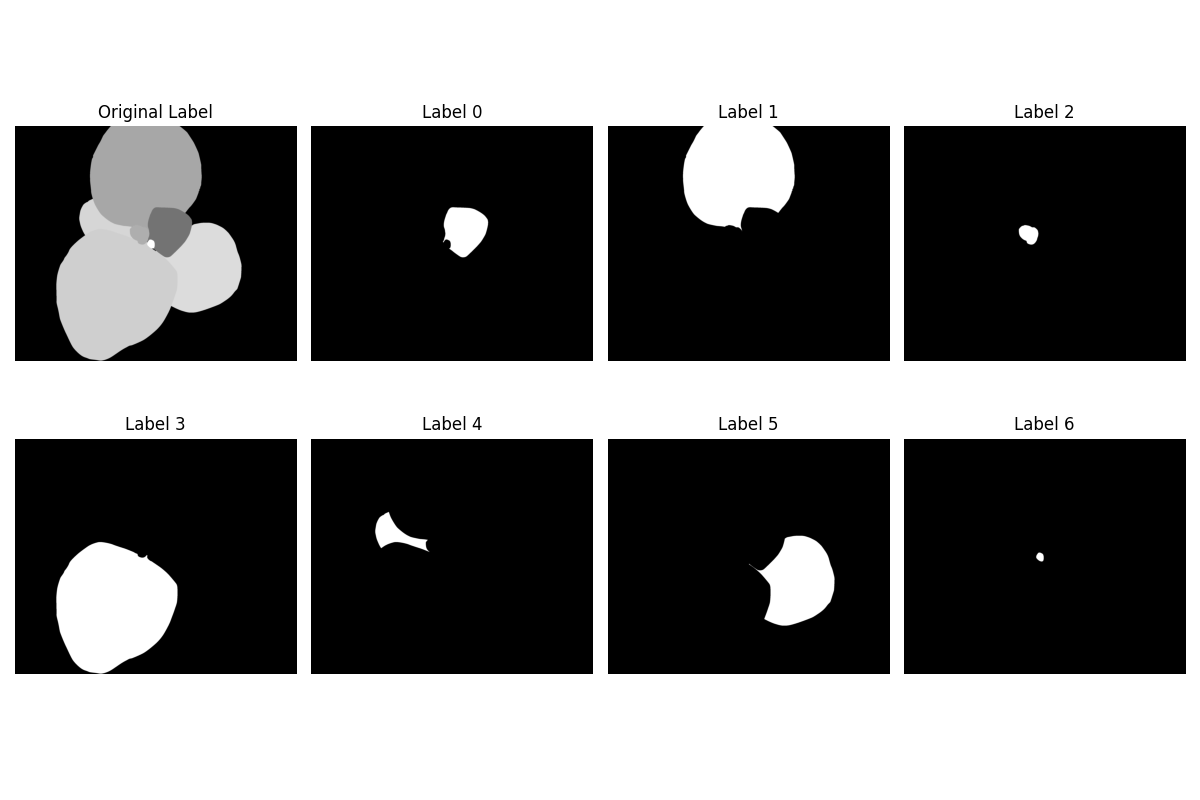
\includegraphics[width=\linewidth]{img/conversion_1.png}
    \caption{Pick single leaves}
    \label{fig_conversion_1}
\end{figure}

To find the contours of the leaves, we can use \verb|cv2.Canny| or \verb|cv2.findContours|. But as the model only need a few points describing the contours, we pick \verb|cv2.findContours| with parameter \verb|method| set to \verb|cv2.CHAIN_APPROX_SIMPLE| and \verb|mode| set to \verb|cv2.RETR_EXTERNAL|. This will generate a series of points denoting a polygon which contains the leaf. The figure \ref{fig_conversion_2} shows the result of label 2 in the figure \ref{fig_conversion_1}.

\begin{figure}[h!]
    \centering
    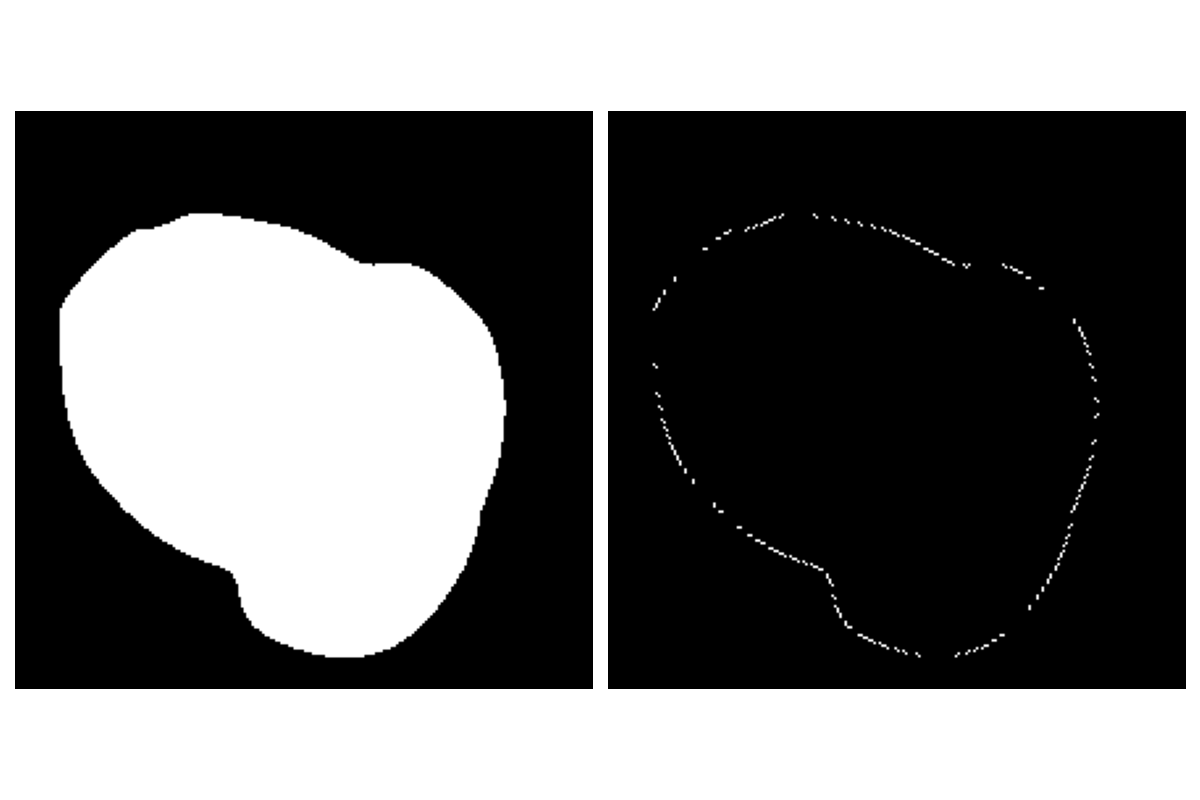
\includegraphics[width=0.75\linewidth]{img/conversion_2_label_2_scaled_up.png}
    \caption{After Processing }
    \label{fig_conversion_2}
\end{figure}

After we got the contours, we can just pick the points in the image and then put them into the JSON file, the preparation of the training data is done.

The second problem is the evaluation. Because we performed the conversion from label images to JSON file, we don't know the relationship of the labels between the output of the model and given labels. Also, the model is not giving us any information about the relation needed for evaluation - which colour maps back to which section of the JSON file. 

Finally, we found the model provided us with the \verb|COCOEvaluator|, which uses the Intersection over Union (\textbf{IoU}) to do the assessment. 

\begin{equation}
    J(A,B)=\frac{|A\cap B|}{|A\cup B|}
    \label{eq:IoU}
\end{equation}

You can see this evaluation is pretty close to \textbf{Dice's coefficient}. 

\begin{equation}
	DSC = \frac{2|X \cap Y|}{|X| + |Y|}
	\label{eq:Dice}
\end{equation}

So we looked into the source code of the \verb|COCOEvaluator| and we found a function called \verb|pairwise_iou| which evaluates the result with equation 1. This makes things easier, we can create a \verb|DiceEvaluator| by replacing different function. But we don't want to modify the source code because this makes code harder to maintain. So we created a class called \verb|DiceEvaluator| which inherits the \verb|COCOEvaluator| and a function called \verb|pairwise_dice| which replaces the \verb|pairwise_iou|. 

Though this solution provides us with some flexibility, we are not having fully control over the output. We used the \verb|redirect_stdout| to change the default output. 


\section{Results and Discussion}

\subsection{Task 1}
For the first task, Let us show the result first. While counting plants, results for Ara2012 and Canon datasets are good, shown in figure \ref{task1_plant_count}, the first line is the number of plants in Ara2012, the second line is for Canon and the third line is for RPi. As you can see, results for Ara2012 is almost perfect. The last picture’s mistake is because two plants’ leaves get too close to each other, so the program regards two plants as one plant

When it comes to Canon dataset, the result is not bad. You can see for the first 6 images, the number of plants is more than 24(there are 24 plants in each image). The most common mistake appears in Canon dataset is shown in Figure \ref{fig:task1_eg_mis_class}, and its hsv image Figure \ref{fig:task1_eg_mis_class} will show you how this mistake happens, although the pot’s edge seems really different in normal(rgb) way, while changing the color area to hsv, it’s easy to mix pot and plants together, because part of 
the pot’s edge is green. And this is what we mentioned before, this size of the wrong bounding boxes may probably  bigger than the baby plants, so this mistake can’t be solved by setting a minimum size.

\begin{figure}[h!]
\centering
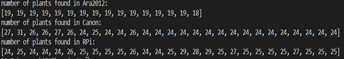
\includegraphics[width=0.9\linewidth]{img/task1_plant_count.png}
\caption{Plant Count}
\label{task1_plant_count}
\end{figure}
\begin{figure}[h!]
\centering
\begin{subfigure}[h!]{0.24\textwidth}
    \centering
    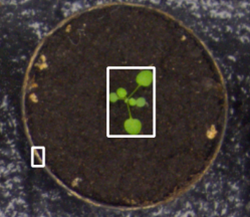
\includegraphics[width=\textwidth]{img/task1_mis_classification.png}
\end{subfigure}
\hfill
\begin{subfigure}[h!]{0.24\textwidth}
    \centering
    \includegraphics[width=\textwidth]{img/task1_mis_classification_enhanced.jpg}
\end{subfigure}
\caption{Wrong area counted}
\label{fig:task1_eg_mis_class}
\end{figure}

Fortunately, when plants grow bigger, the average size of plants increases. So this kind of noise will be too small to be detected, you can see in the last 16 images, no error happens in figure \ref{task1_plant_count}.  
	As for RPi dataset, the result not as good as Canon’s, you can see only 6 images are considered to have 24 plants. The most common errors are shown in Figure \ref{fig:task1_good_eg}. In Figure\ref{fig:task1_good_eg}, a hsv image is shown, it’s obvious that the plant’s stem and pot has the same color, so in RPi dataset, the biggest challenge comes from pot, not moss. This is because the light changes in different datasets - RPi dataset is brighter than Canon dataset. 
    
\begin{figure}[h!]
\centering
\begin{subfigure}[h!]{0.24\textwidth}
    \centering
    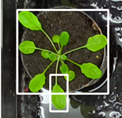
\includegraphics[width=\textwidth]{img/task1_good_class.png}
\end{subfigure}
\hfill
\begin{subfigure}[h!]{0.24\textwidth}
    \centering
    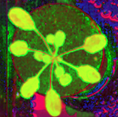
\includegraphics[width=\textwidth]{img/task1_good_class_enhanced.png}
\end{subfigure}
\caption{When works properly}
\label{fig:task1_good_eg}
\end{figure}
To wipe out pot’s noise, no red is allowed to show up, but this will damage part of the stem and create an disconnected part: a leaf. What’s worse, these disconnected leaves are even bigger than baby plants, which makes it really hard to filter out. 

To solve this problem, we turn to rgblab, hope can have a better result. The result shown in Figure \ref{task1_no_pot} seems perfect, this is the result of using rgblab color space. But if you take a close look, although pot is obviously different from leaves, stem’s color is similar to some background noise. We finally choose hsv because background noise is more disgusting and harder to filter, it brings more errors.

\begin{figure}[h!]
\centering
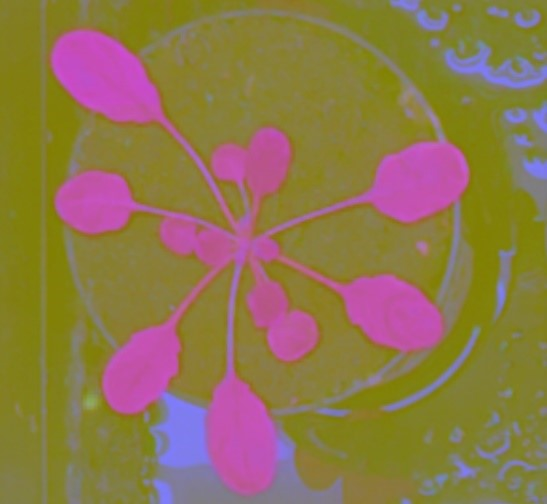
\includegraphics[width=0.7\linewidth]{img/task1_no_pot.jpg}
\caption{Foreground}
\label{task1_no_pot}
\end{figure}

The average precision of these three datasets are shown in figure \ref{task1_eva}. You can see even we get some mistakes, the accuracy is still high, which means our solution works fine.


\begin{figure}[h!]
\centering
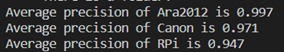
\includegraphics[width=0.7\linewidth]{img/task1_eva.png}
\caption{Result}
\label{task1_eva}
\end{figure}

\subsection{Task 2}
We convert RGB image to HSV color space and apply medium filter for denoising, for most runs, results are shown to be over 95 DSC, 90 IOU, which is a very high accuracy rate. The sample image after extracting green color is shown in figure \ref{task2_binary_graph_after_extracting_green_color}

\begin{figure}[h!]
\centering
\includegraphics[width=0.9\linewidth]{img/task2_binary_graph _after_extracting_green_color.png}
\caption{Binary graph after extracting green color}
\label{task2_binary_graph_after_extracting_green_color}
\end{figure}
Also, image after medium filtering, as shown in Figure \ref{task2_binary_graph_after_medium_filtering} below:

\begin{figure}[h!]
\centering
\includegraphics[width=0.9\linewidth]{img/task2_binary_graph_after_medium_filtering.png}
\caption{Binary graph after medium filtering}
\label{task2_binary_graph_after_medium_filtering}
\end{figure}
DSC and IOU result is shown in Figure \ref{task2_dice_and_iou}

\begin{figure}[h!]
\centering
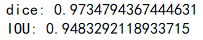
\includegraphics[width=0.5\linewidth]{img/task2_dice_and_iou.png}
\caption{Evaluation result of sample image}
\label{task2_dice_and_iou}
\end{figure}

Overall, these results indicate that color space methods have positive effects in this experiment. In the process, adjusting the value of HSV is a very important point. According to observations, the green components in the soil are generally deeper than the plants themselves; therefore the brightness threshold can be adjusted to obtain a better filtering effect. For filtering, it is necessary to select a method and parameters suitable for the shape of the picture. Otherwise, there are many methods that are also considered effective to accomplish this task, such as training a classifier. Also in \verb|opencv-python|, using the rectangle function to frame the plants seems to be a way to get more accurate results. In this experiment, however, there are still a lot of green impurities in the plant frame so the actual effect is not ideal. Hope to have further development in image segmentation algorithm.

\subsection{Task 3 Instance Segmentation}

The \verb|TensorBoard| is used to visualize our training process.
Shown on Fig.\ref{fig:loss for training process}.
During the increase of iterations, the model gets stable.
And the total loss drops ideally.

\begin{figure}[h!]
\centering
\begin{subfigure}[h!]{0.24\textwidth}
    \centering
    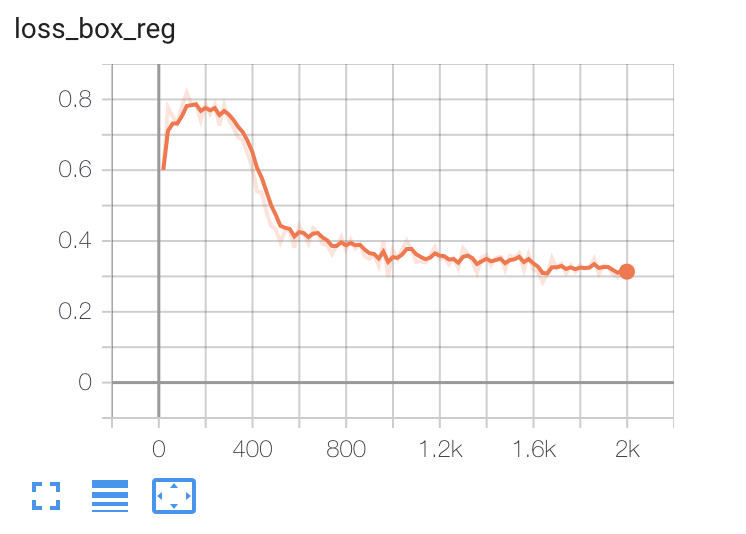
\includegraphics[width=\textwidth]{img/loss_bbox_reg.png}
    \caption{bbox regression loss}
    \label{fig:loss_bbox}
\end{subfigure}
\hfill
\begin{subfigure}[h!]{0.24\textwidth}
    \centering
    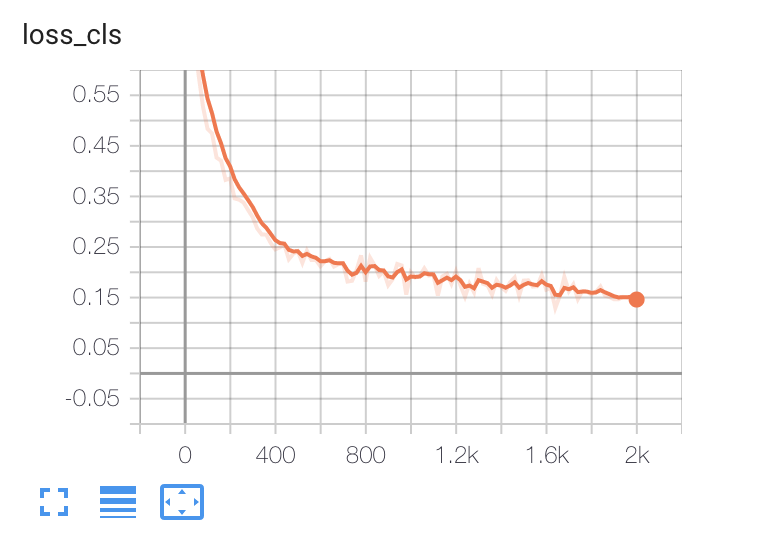
\includegraphics[width=\textwidth]{img/loss_cls.png}
    \caption{classification loss}
    \label{fig:loss_cls}
\end{subfigure}
\hfill
\begin{subfigure}[h!]{0.24\textwidth}
    \centering
    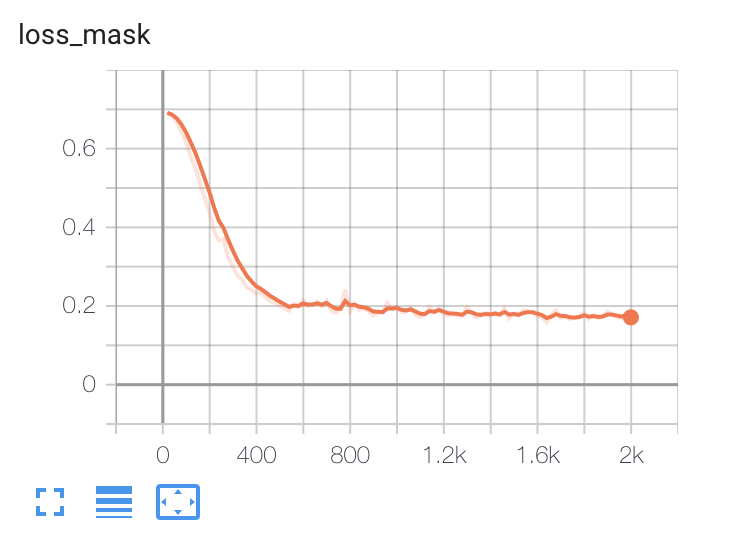
\includegraphics[width=\textwidth]{img/loss_mask.png}
    \caption{mask loss}
    \label{fig:loss_mask}
\end{subfigure}
\hfill
\begin{subfigure}[h!]{0.24\textwidth}
    \centering
    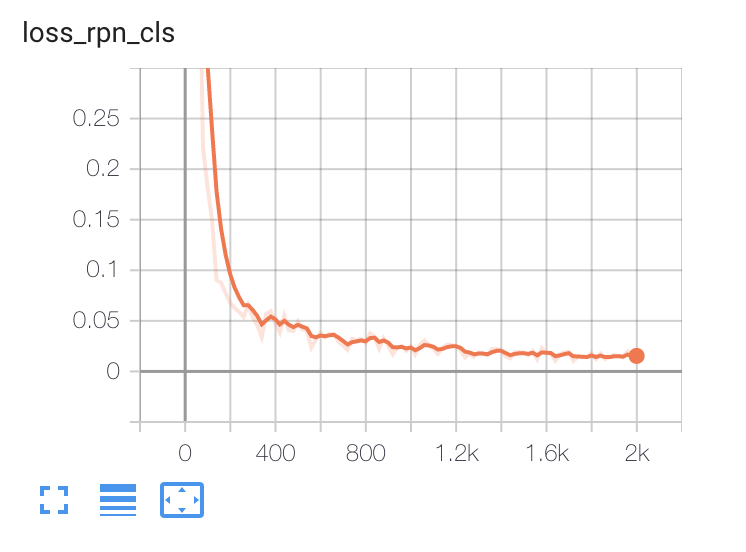
\includegraphics[width=\textwidth]{img/loss_rpn_cls.png}
    \caption{RPN classification loss}
    \label{fig:loss_rpn_cls}
\end{subfigure}
\hfill
\begin{subfigure}[h!]{0.24\textwidth}
    \centering
    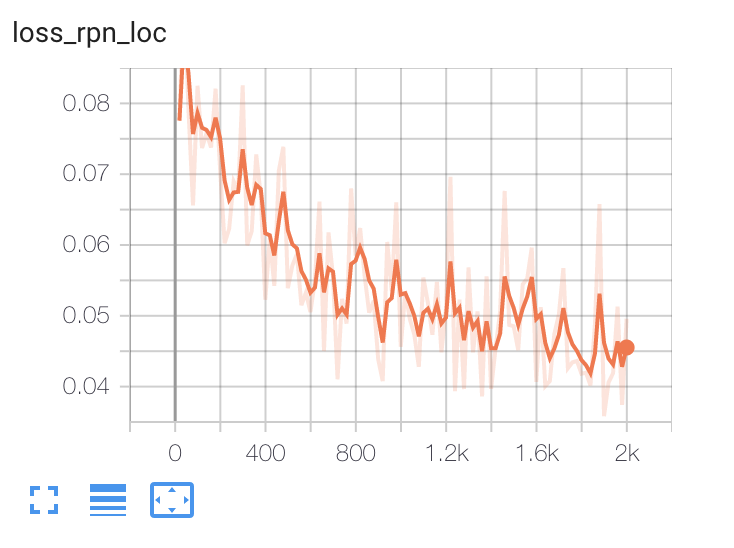
\includegraphics[width=\textwidth]{img/loss_rpn_loc.png}
    \caption{RPN loc loss}
    \label{fig:loss_rpn_loc}
\end{subfigure}
\hfill
\begin{subfigure}[h!]{0.24\textwidth}
    \centering
    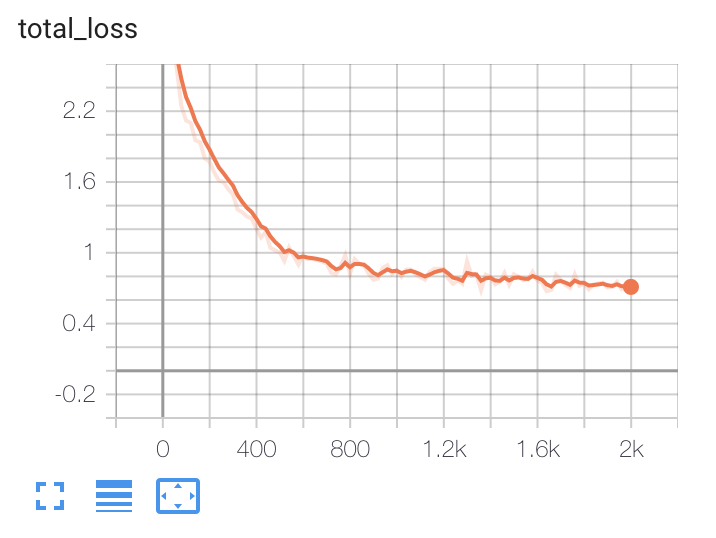
\includegraphics[width=\textwidth]{img/loss_total.png}
    \caption{total loss}
    \label{fig:loss_total}
\end{subfigure}
   \caption{loss for training process}
   \label{fig:loss for training process}
\end{figure}

\begin{figure}[h!]
    \centering
    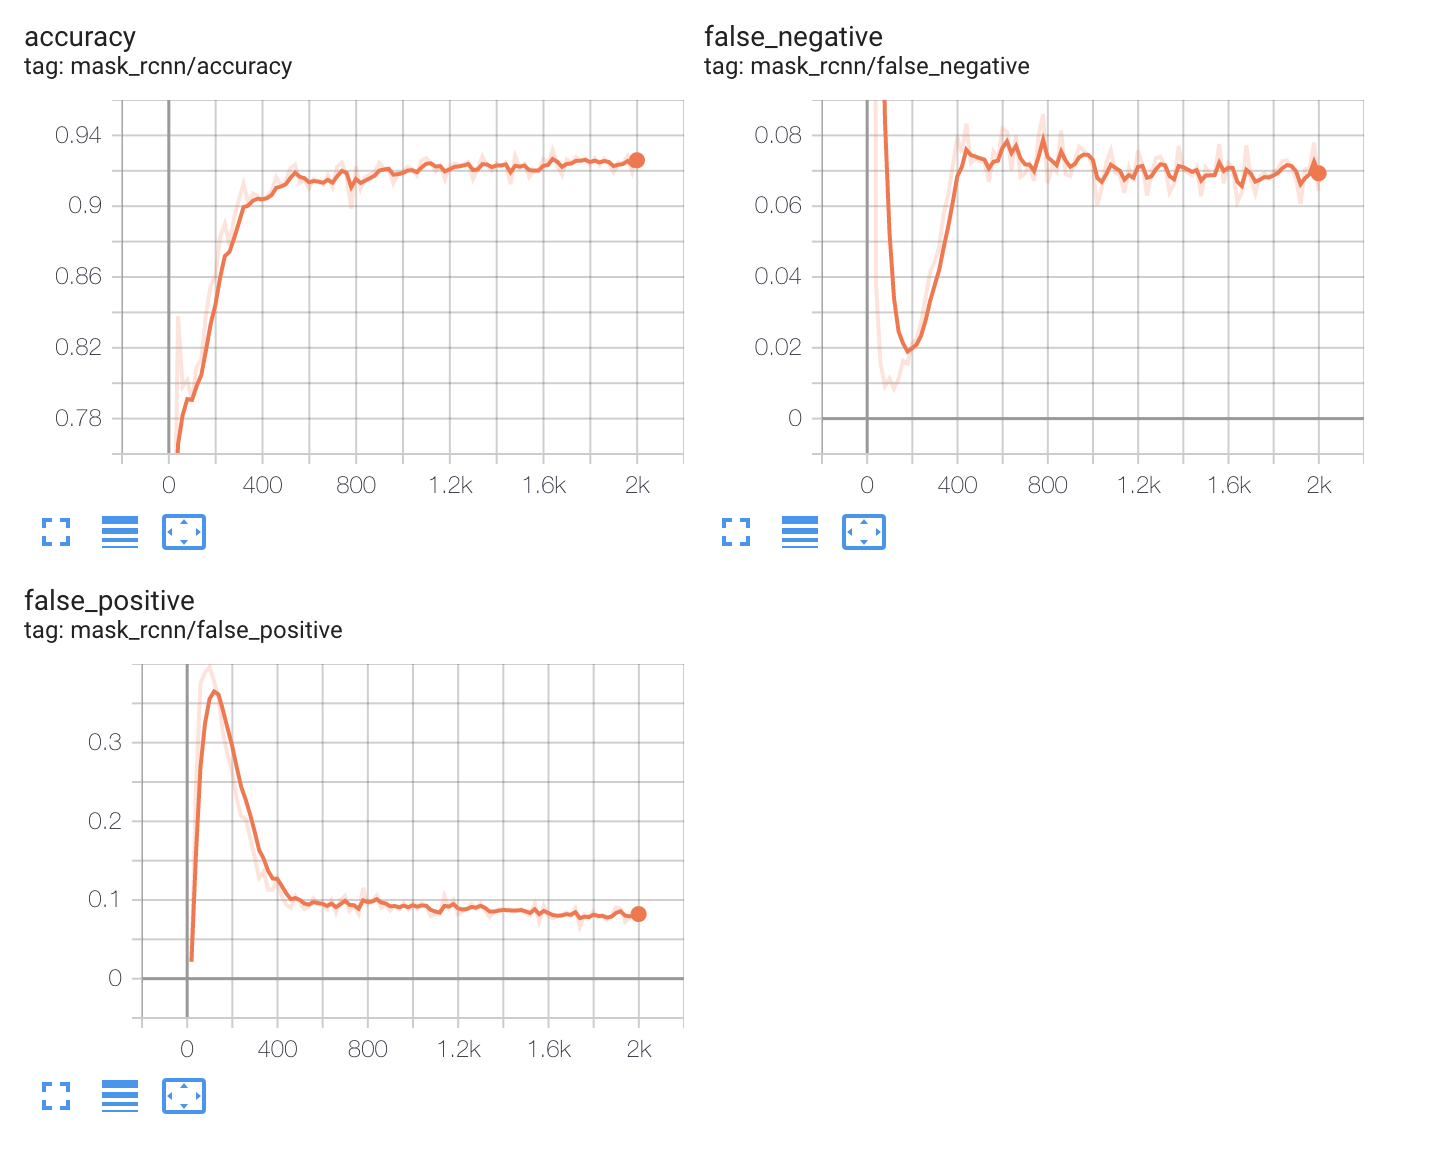
\includegraphics[width=\linewidth]{img/ap_maskrcnn.png}
    \caption{Mask RCNN}
    \label{fig_ap}
\end{figure}

Here are some prediction results. Refer to Fig. \ref{fig:prediction}.
This result of this model shows quite well. 

\begin{figure}[h!]
\centering
\begin{subfigure}[h!]{0.24\textwidth}
    \centering
    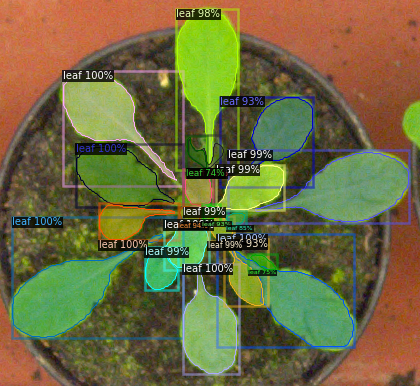
\includegraphics[width=\textwidth]{img/pred1.png}
    % \caption{loss bbox regression}
    % \label{fig:loss_bbox}
\end{subfigure}
\hfill
\begin{subfigure}[h!]{0.24\textwidth}
    \centering
    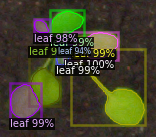
\includegraphics[width=\textwidth]{img/pred2.png}
    % \caption{loss classification}
    % \label{fig:loss_cls}
\end{subfigure}
\hfill
\begin{subfigure}[h!]{0.4\textwidth}
    \centering
    \includegraphics[width=\textwidth]{img/pred3.png}
    % \caption{loss mask}
    % \label{fig:loss_mask}
\end{subfigure}
\caption{Prediction samples}
\label{fig:prediction}
\end{figure}

However, there are still some images not fit well. Refer to Fig.\ref{fig:bad_result}.
Especially these images with low resolution, some leaves do not have a clear boundary,
and some leaves are overlapped with each other. Even human beings cannot distinguish that.

\begin{figure}[h!]
\centering
\begin{subfigure}[h!]{0.24\textwidth}
    \centering
    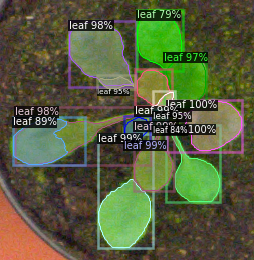
\includegraphics[width=\textwidth]{img/ara2012_plant009.png}
    % \caption{loss bbox regression}
    % \label{fig:loss_bbox}
\end{subfigure}
\hfill
\begin{subfigure}[h!]{0.24\textwidth}
    \centering
    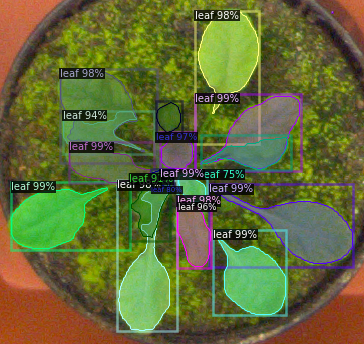
\includegraphics[width=\textwidth]{img/ara2012_plant110.png}
    % \caption{loss classification}
    % \label{fig:loss_cls}
\end{subfigure}
\hfill
\begin{subfigure}[h!]{0.24\textwidth}
    \centering
    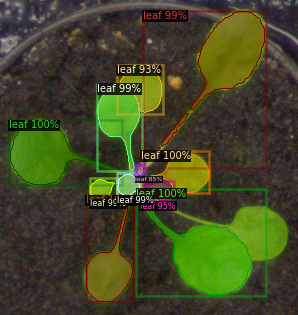
\includegraphics[width=\textwidth]{img/ara2013_plant162.png}
    % \caption{loss mask}
    % \label{fig:loss_mask}
\end{subfigure}
\caption{Some sample images show not so well}
\label{fig:bad_result}
\end{figure}

\begin{figure}[h]
    \centering
    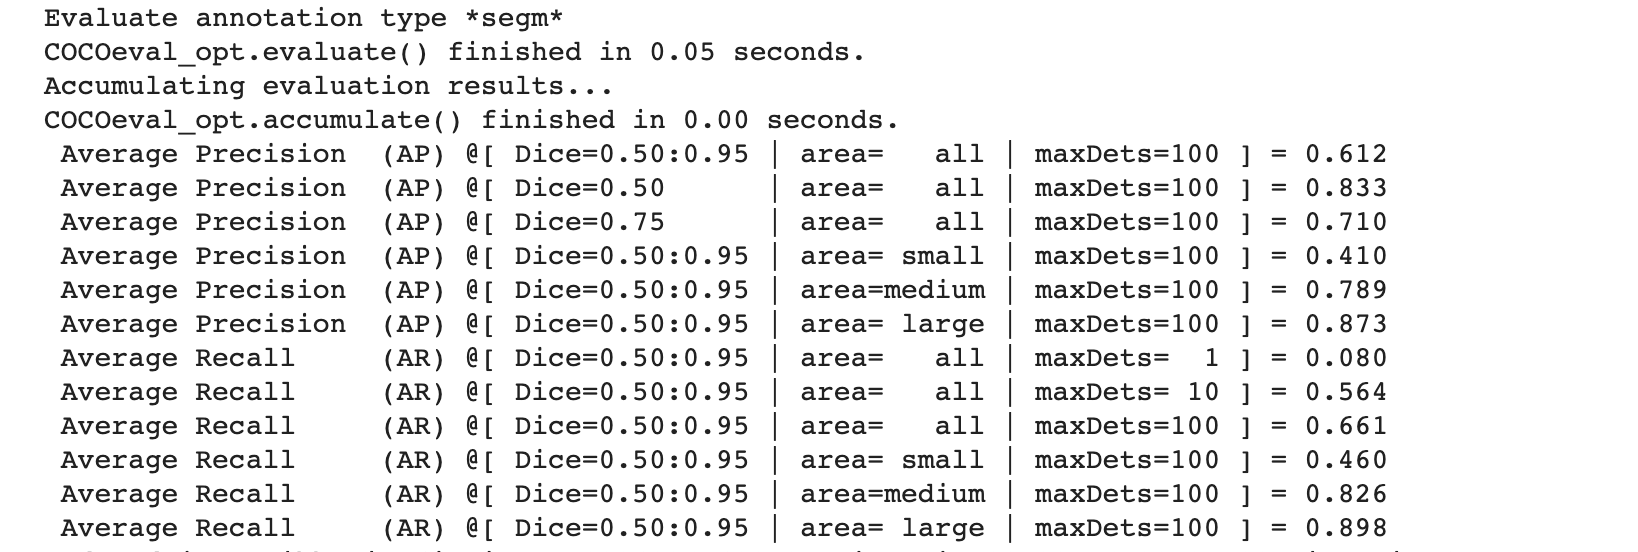
\includegraphics[width=\linewidth]{img/dice_evl.png}
    \caption{Evaluation Dice}
    \label{fig_ap}
\end{figure}


\section{Conclusion}

From these three datasets, it’s clear that using color extracting is not a good choice for task 1. Even with the same plants, results would be different if the light gets brighter or darker. Noise from other plants and soil or other kinds of background are also harmful to results. So we strongly recommend not to use color extracting while dealing with these sort of projects. The same situation also happened to task 2. The task 3 used deep learning method. Though the results are mostly satisfying, the model is more complicated to be understand. 

And the last thing I want to mention about is the team working. Through this teamwork, every member has benefited a lot. This time we used Github to achieve effective and high-speed processing of project version management. Though some members on the team were not familiar with Github at first, they gradually learned to upload codes, create branches, push updates, etc., which are very helpful for future project collaboration. At the beginning we assigned 3 tasks to members independently, everyone completes their own part. But as the project progressed, the correlation and dependency between the tasks were discovered and mined, then we increased the communication between the teams, which greatly improved the efficiency. For instance, task2 can use the method of task1 to frame plants as a solution to increase accuracy. In the whole process, however, we also encountered many difficulties. When merging the codes and the report, the format inconsistency took us much time to reformat. This also makes us realize that it is important to regulate a unified standard at the beginning of a team project. All in all, this project has not only improved our professional knowledge and application capabilities in computer vision, but also increased our experience in teamwork. 

\section{Contribution of Group Members}

our repo: \url{https://github.com/SolariaProject/COMP9517_Project.git}

All the commit information can be found in this repo git log.

Task 1: Yue He
Task 2: Mingxi Shen, Mingqian Lin
Task 3: Yishun Jin, Wei Wang


\bibliographystyle{IEEEtran}
\bibliography{mybib}


\end{document}


